\subsection{Overordnet}\label{sec:designOverordnet}
% Magnus
% Hvordan startes spillet? 
\textbf{Start:} I \textsc{AvaDam} startes spillet ved at spilleren trykker \texttt{"Start new game"} i main menuen, som set i figur \ref{fig:gameStart}. Derefter oprettes et model objekt i \texttt{View} klassen. Brikker og felter oprettes som objekter af typerne \texttt{Piece} og \texttt{Tile}, der er fields i modelobjektet. I \textsc{SimpDam} startes spillet direkte, når programmet åbnes.

    \begin{figure}[H]
        \centering
        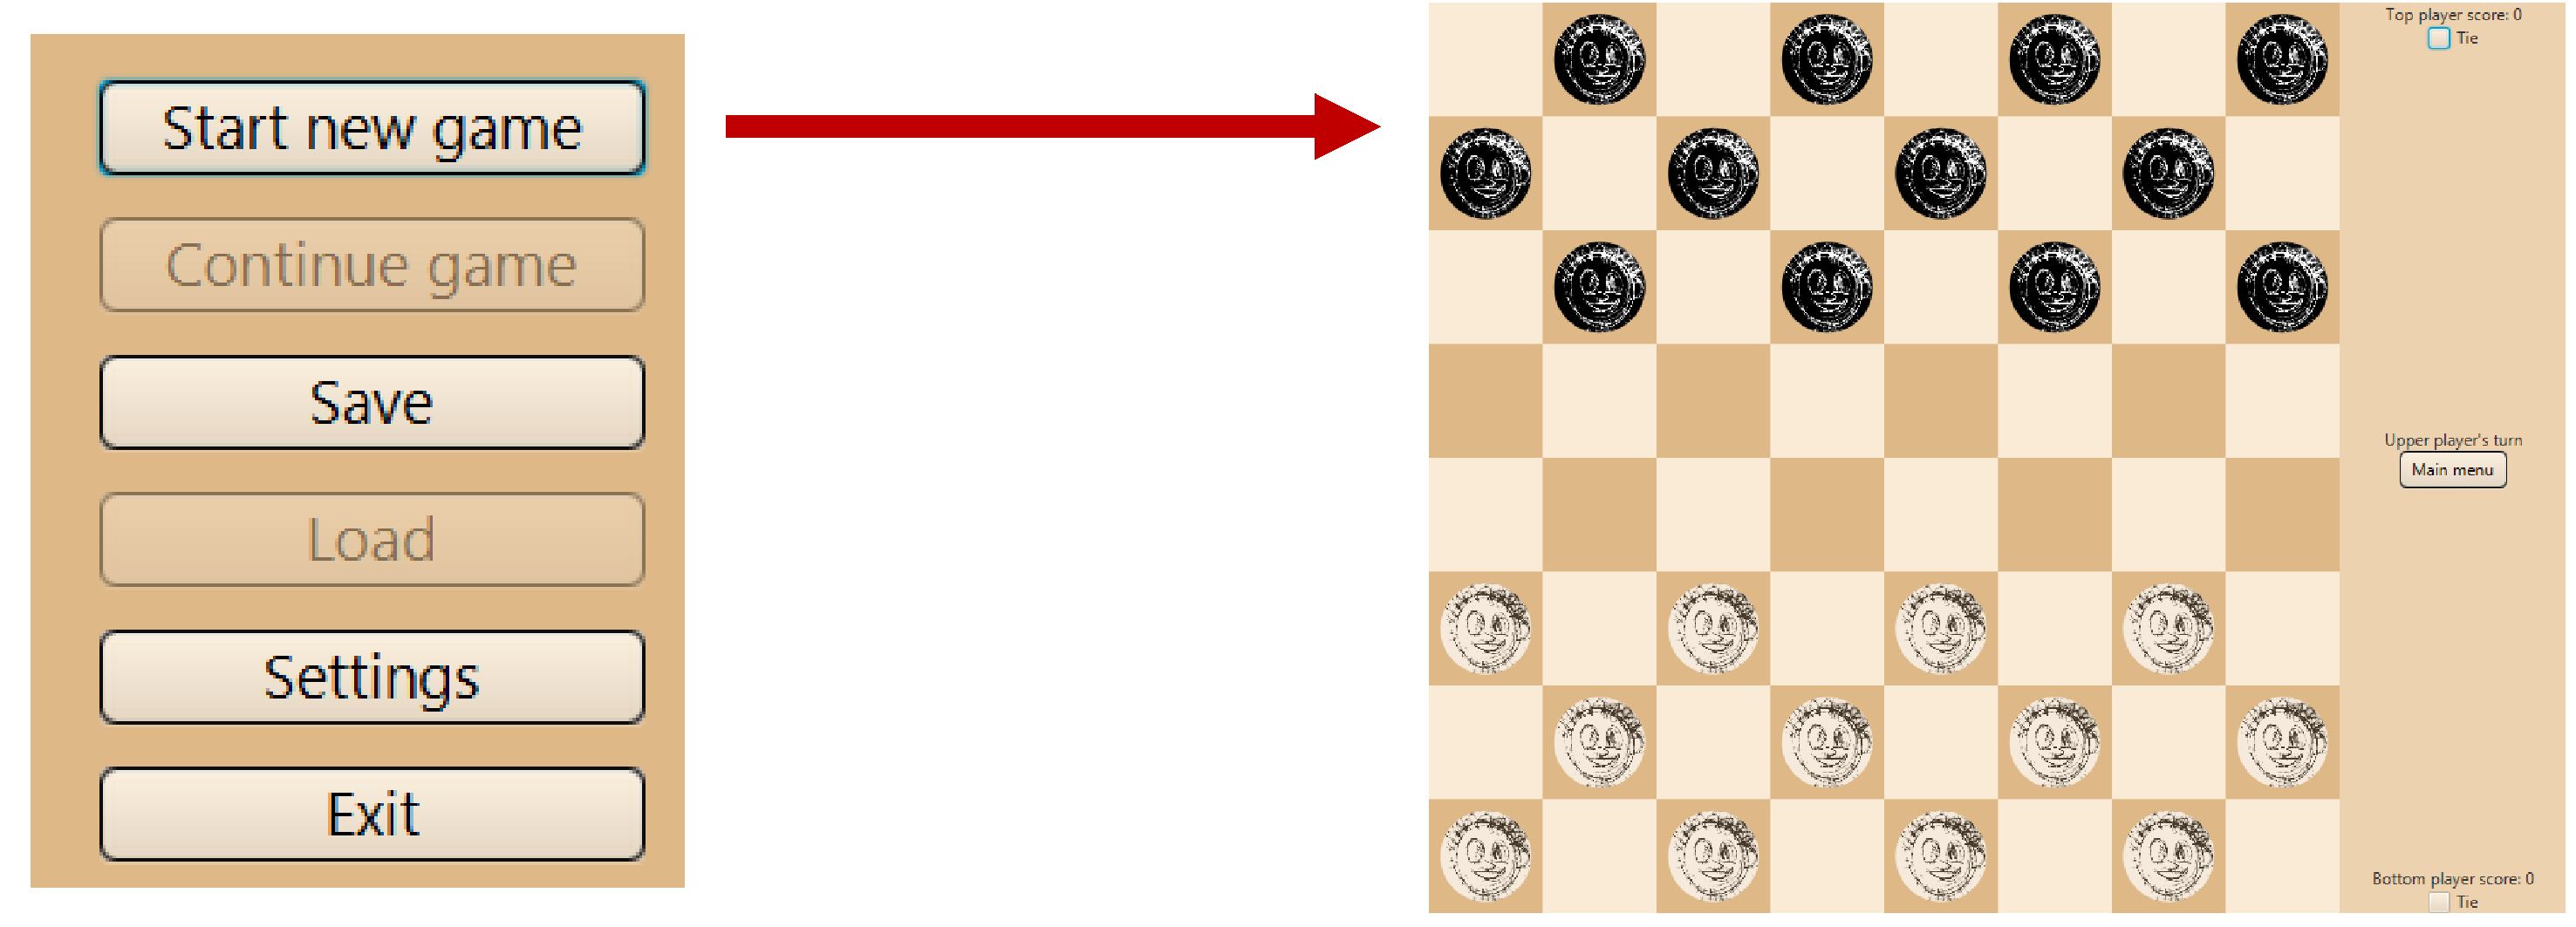
\includegraphics[width = 0.7  \textwidth]{Figurer/gameStart}
        \caption{Overgang fra main menu scenen til spil scenen når spillet startes. Her med standard størrelse 8x8.}
        \label{fig:gameStart}
    \end{figure}

% Magnus
% Hvordan ved jeg, hvis tur det er?
\textbf{Tur:} Spilleren får vink om, hvorvidt det er deres tur. I \textsc{SimpDam} kan du kun trække i dine brikker, når det er din tur. I \textsc{AvaDam} benyttes en del visuelle vink; Modstanderens brikker bliver lidt gennemsigtige. Når du trækker en brik, farves legale felter, du kan flytte til. I panelet til højre står også, hvilken spiller der har tur. Når der spilles mod en AI, animeres AI'ens træk. Disse features uddybes senere. En variabel, der indeholder hvis tur det er, lagres i en klassen \texttt{Control}, i field af typen \texttt{Player} (\texttt{enum} med \texttt{mulighederne Upper, Lower, None}).\\

% Magnus
% Hvordan flytter jeg en brik?
\textbf{Flytning af brik:} Brikker flyttes ved at trække musen, dvs.: Klik ned på brikken du vil flytte, træk til slutfeltet, slip musen. Når brikken tages op, opdateres fields i \texttt{Control}, der benyttes i senere metoder. Når brikken trækkes, tegnes brikken kontinuerligt, dvs. brikken følger med musen. Når spilleren slipper brikken over et felt, køres metoder gennem i klasserne \texttt{TopLevelControl} og \texttt{Control}\footnote{I \textsc{AvaDam} tjekkes også om et felt er en legal midlertidig destination i en combo}. Disse metoder tjekker om trækket var legalt.
\\

%   RR
% \item Kan man ombestemme sig, når man flytter brik? (før flyt er sket) Hvordan? (begge)
\textbf{Fortrydelse af valgt brik:} 
Så snart en brik er sluppet vil den enten få den nye position hvis det er et legalt træk, ellers sat tilbage på den originale plads. Dette gør det meget nemt at fortryde et træk da man kan slippe den hvor som helst, så længe det ikke indgår i et legalt træk. Ved at trækket var illegalt er det stadig den samme spillers tur. På den måde bliver det meget intuitivt og nemt at vælge en anden brik / vælge et andet træk. \\

% Magnus
% Virker spillet med touch screen?
\textbf{Touch screen:} Spillet virker ikke med touch screen, da touch screen mussetræk (dragging) og \texttt{JavaFX} ikke samarbejder optimalt. Vores program er afhængigt af at mussetræk påbegyndes og afsluttes, da vi anvender \texttt{setOnMouseClicked}, \texttt{setOnMouseDragged} og \texttt{setOnMouseReleased} fra \texttt{JavaFX}. Med touch screen kan man med hurtige og samtidige mussetræk forvirre \texttt{JavaFX}: \texttt{MouseClicked} kan forekomme uden \texttt{MouseReleased}.\\

% Magnus
% Kan man bruge keyboard til at spille spillet?
\textbf{Keyboard:} Keyboardet kan bruges i begrænset omfang til spillet. Når brugeren er i spillet, fås main menuen frem ved at trykke escape. Når brugeren er i menuer, kan piletaster og space bruges til interaktion. \\

% Magnus
% Hvad er model og view koordinater?(originalt fra implementering)
\textbf{Model og view koordinater:} I modellen findes et array \texttt{Tile}$[\, \, \,][\, \, \,]$ \texttt{board}, der lagrer brættets felter. Indekserne i board i hhv. x- og y-retning kaldes model koordinater, dvs. feltet \texttt{board[0][7]} har model koordinaterne (0,7). Når feltet tegnes i scenen, sker det i stedet på dets view koordinater. View koordinaterne afhænger af variablene \texttt{sceneWidth} og \texttt{sceneHeight}, der sættes i \texttt{View}, når programmet åbnes. De afhænger af skærmens størrelse:
\begin{lstlisting}
static double boardHeight = (Screen.getPrimary().getBounds().getHeight() - 100);
\end{lstlisting}
dvs. alle shapes, der tegnes, er skaleret i forhold til skærmens størrelse. Det gør spillet uafhængigt af skærmens opløsning, og således spilbart på de fleste skærme.\\

 \begin{figure}[H]
        \centering
        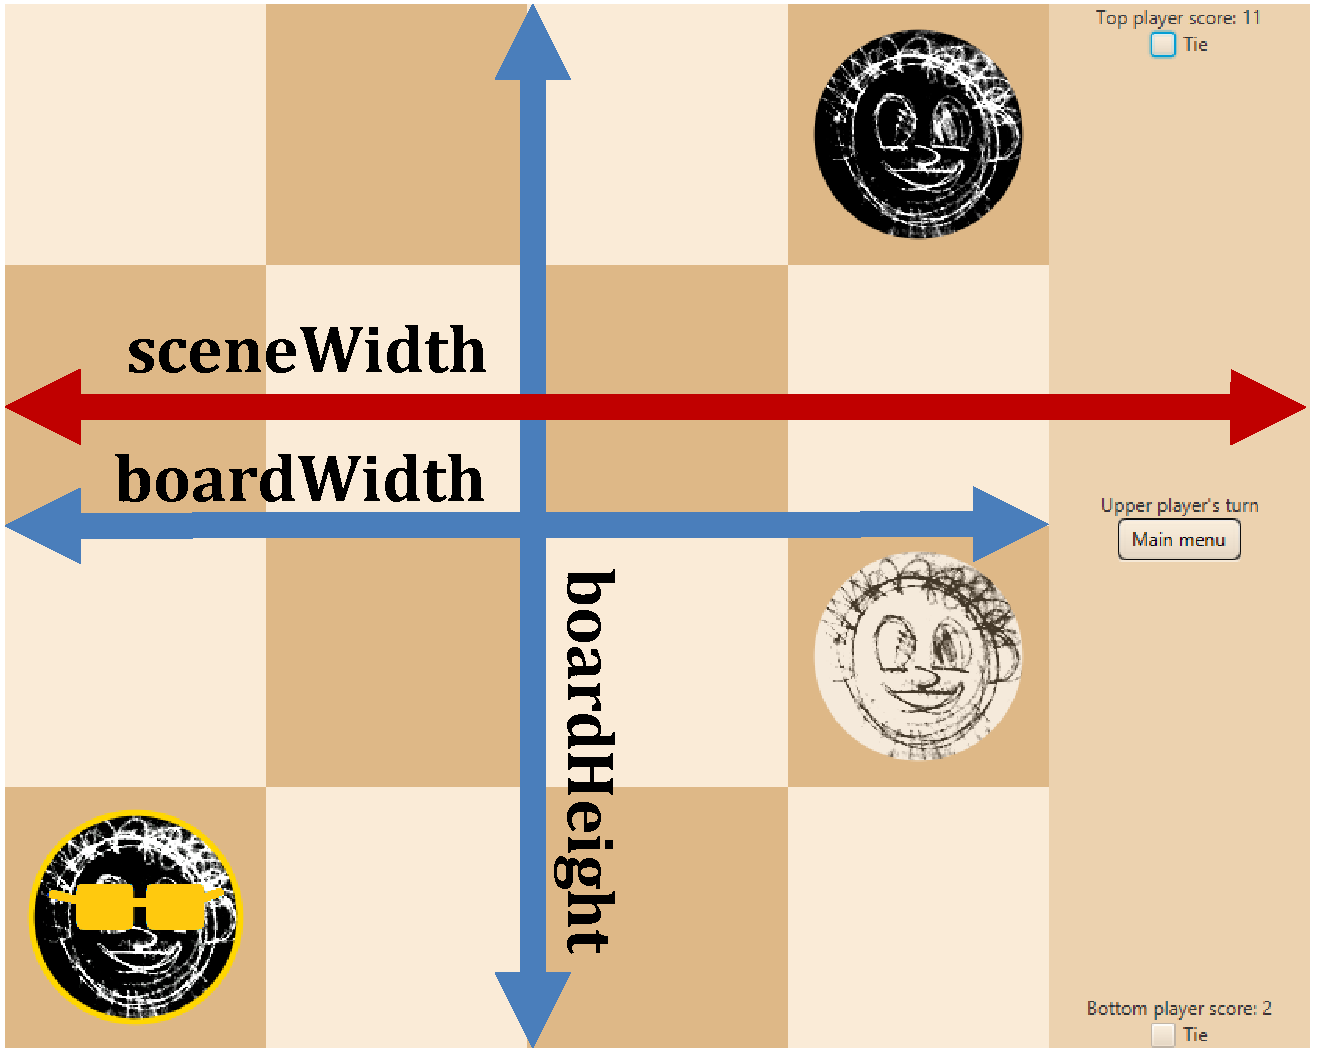
\includegraphics[width = 0.6  \textwidth]{Figurer/heightWidth.pdf}
        \caption{Visuel oversigt over størrelserne af \texttt{boardWidth}, \texttt{boardHeight} og \texttt{sceneWidth}.}
        \label{fig:heightWidth}
    \end{figure}

% Magnus
% Hvilke classes bruger spillet?
\textbf{Klasser:} Programmet bruger 15 klasser, fordelt i 3 kategorier: model, view og control. Klasserne gennemgås i detaljer i kategoriernes respektive afsnit, men i korte træk bruges klasserne i figur \ref{fig:MVC}. Ethvert felt på brættet er af typen \texttt{Tile}. Enhver brik er af typen \texttt{Piece}.
